\documentclass[11pt,a4paper]{article}
\usepackage[T1]{fontenc}
\usepackage[utf8]{inputenc}
\usepackage{lmodern}
\usepackage[english]{babel}
\usepackage{geometry}
\geometry{margin=25mm}
\usepackage{microtype}
\usepackage{amsmath,amssymb,amsthm}
\usepackage{booktabs,longtable,array,tabularx,multirow}
\usepackage{graphicx}
\usepackage{url}
\usepackage{hyperref}
\usepackage{enumitem}
\usepackage{listings}
\usepackage{xcolor}
\usepackage{caption}
\usepackage{float}
\usepackage{fancyhdr}
\usepackage{needspace}
\hypersetup{colorlinks=true,linkcolor=black,citecolor=black,urlcolor=blue,pdftitle={TODM: A Test Oracle-Driven Methodology for Human-Governed AI Software Engineering},pdfauthor={Jose Maria Flores Zazo}}
\setlength{\parskip}{3pt}
\setlength{\parindent}{0pt}
\setlength{\emergencystretch}{2em}
\setlist[itemize]{nosep,leftmargin=1.6em}
\setlist[enumerate]{nosep,leftmargin=1.8em}
\newcommand{\todm}{\textsc{TODM}}
\newcommand{\PASS}{\textsf{PASS}}
\newcommand{\FAIL}{\textsf{FAIL}}
\newcommand{\INC}{\textsf{INCONCLUSIVE}}
\newcommand{\Gate}[1]{\textsf{G#1}}
\newtheorem{definition}{Definition}
\newtheorem{claim}{Design proposition}
\lstdefinestyle{paper}{basicstyle=\ttfamily\small,breaklines=true,columns=fullflexible,frame=single,rulecolor=\color{black!20},showstringspaces=false,keepspaces=true}
\lstset{style=paper}
\pagestyle{fancy}\fancyhf{}\fancyhead[L]{\small Test Oracle-Driven Methodology (TODM)}\fancyhead[R]{\small Methodology and evaluation protocol}\fancyfoot[C]{\thepage}\renewcommand{\headrulewidth}{0.3pt}
\title{\textbf{TODM: A Test Oracle-Driven Methodology for Human-Governed AI Software Engineering}\\[5pt]\large A Tool-Agnostic, Falsifiable Method for Greenfield Development, Brownfield Modernization, and Application Management}
\author{Jos\'e Mar\'ia Flores Zazo}
\date{28 October 2026 --- Research artifact companion, v1.5}
\begin{document}
\maketitle
\vspace{-1.3em}
\begin{abstract}
Generative coding agents can derive specifications, tests, and software from the same interpretation of requirements. They may therefore agree with one another while still violating an authoritative business rule. We introduce the Test Oracle-Driven Methodology (TODM), a tool-agnostic engineering method that separates human approval of expected behavior from AI-delegated software construction and independent verification. TODM defines a versioned, approved oracle baseline; three governance, construction, and verification planes; eight lifecycle gates with explicit recovery paths; and three-valued verification outcomes (PASS, FAIL, INCONCLUSIVE). It composes, as needed, five established modeling families: business vocabulary and rules (SBVR), decisions (DMN), processes (BPMN), cases (CMMN), and invariants (OCL). We specify the authority and evidence requirements for executable oracles, show how mutation testing can qualify the oracles themselves, and illustrate a shared-specification error that may escape agent-generated tests. The method covers greenfield development, brownfield modernization, and Application Management Services (AMS), including incremental replacement and single-cutover migration. We define measurable quality and autonomy metrics and a controlled comparative evaluation protocol. We also distinguish the authorization of agent actions from the behavioral correctness of their outputs, and specify how TODM can interoperate with constitutional and polycentric agent governance without depending on it. This manuscript specifies falsifiable claims and includes a synthetic engineering acceptance artifact; it reports no comparative empirical effectiveness results or guarantees of autonomous performance.
\end{abstract}
\noindent\textbf{Keywords:} test oracle problem; software engineering methodology; AI coding agents; model-based testing; human oversight; agent governance; legacy modernization; software maintenance; mutation testing; behavioral contracts.

\section{Introduction}
Agentic coding systems increasingly support specification, design, source-code production, testing, refactoring, and repair. These capabilities change how software is produced, but do not eliminate the question of how a team can establish the expected behavior independently of the implementation. The \emph{test oracle problem} is the challenge of deciding whether an observed response is correct \cite{barr2015oracle}. Its relevance grows when the same agent, model family, prompt context, or generated specification supplies both the software and the examples used to approve it.

Consider a sales authorization rule. A signed business policy requires human review for requests above EUR~10,000. An agent mistakenly records EUR~12,000 in the generated specification; subsequent code and tests follow that threshold. Traditional unit tests, business examples, and specification-consistency checks may all pass. A request of EUR~11,000 is nevertheless incorrectly authorized. The defect arises not merely from inadequate test quantity, but from an inadequate source of expected outcomes and weak separation of approval authority.

\todm{} is proposed to address this governance-and-verification failure mode. It organizes work around \emph{approved, independently executed behavioral oracles}, not around a specific programming assistant, framework, process engine, or migration strategy. An oracle is not just a test case: it is a rule with an accountable source, declared semantics, required observations, evaluation logic, and auditable evidence. Agents may propose an oracle, but the implementation agent must not be able to unilaterally approve or rewrite the authority against which its output is assessed.

This article provides: (C1) an operational definition of an approved oracle baseline; (C2) an eight-stage, artifact-driven method with explicit gates and reverse transitions; (C3) a verification-plane architecture integrating five risk-selected model families; (C4) a reference tri-valued acceptance semantics and controls to test the oracles themselves; and (C5) a falsifiable research protocol; and (C6) an explicit authority-versus-correctness separation for integration with external agent governance. These are \emph{proposed contributions}, not claims of unprecedented components or experimentally proven superiority.

\section{Foundations and Related Work}
\subsection{The established oracle problem}
Barr et al.'s 2015 survey synthesizes long-standing oracle techniques, including specifications, models, contracts, and metamorphic relations \cite{barr2015oracle}. Mutation testing deliberately injects faults to evaluate whether tests can distinguish faulty variants \cite{jia2011mutation}; metamorphic testing checks relations between executions when individual expected outputs are difficult to specify \cite{segura2016metamorphic}. \todm{} relies on these precedents. It does not claim to invent test oracles, model-based testing, human approval, or mutation testing.

\subsection{Specifications, example-driven testing, and software construction}
Specification-driven development structures the path from intent to implementation; modern tooling such as GitHub Spec Kit includes specification, planning, tasks, implementation, and convergence as well as optional consistency controls \cite{github2026speckit}. Test-driven development and behavior-driven development help developers express and exercise expected outcomes; Gherkin offers a common language for executable examples \cite{cucumber2026}. \todm{} is \emph{complementary}: a vetted specification or example can itself become an oracle. The method's additional requirement is independent authority over the behavioral contract, explicit qualification of its defect-detection ability, and sustained verification against system observations. It would be inaccurate to argue that SDD, TDD, or BDD inherently prevent such controls; their implementations can incorporate them.

\subsection{Legacy characterization and modernization strategy}
Legacy characterization tests document observed behavior, helping engineers change unfamiliar systems \cite{feathers2004legacy}. Yet observation does not prove business correctness: historical defects may be copied into a replacement system. Incremental replacement patterns, such as the Strangler Fig approach, offer deployment choices rather than a comprehensive theory of behavioral truth \cite{fowler2004strangler}. \todm{} separates normative requirements, observed legacy behavior, and machine-inferred hypotheses and permits incremental or single-cutover delivery.

\subsection{Modeling standards and executable tools}
The Object Management Group publishes standard descriptions for business processes (BPMN), cases (CMMN), decisions (DMN), business rules and vocabulary (SBVR), and constraints (OCL) \cite{omg2014bpmn,omg2016cmmn,omg2024dmn,omg2019sbvr,omg2014ocl}. Existing engines, including Flowable, execute significant BPMN, CMMN, and DMN subsets \cite{flowable2026}. TODM therefore specifies \emph{adapters and supported semantic profiles}, not five novel universal standards implementations. A Mermaid diagram, JSON document, or YAML file is not automatically an OMG-compliant execution model. Model syntax, version, supported constructs, and runtime behavior must be declared.

\subsection{Research positioning and the novelty boundary}
The constituent techniques are established, and systems that combine AI modernization, knowledge extraction, human oversight, and rule engines exist. Consequently, neither a claim of a globally unprecedented architecture nor a claim that no competing methodology exists can be substantiated by this paper. The specific research contribution is an \emph{explicitly specified methodological composition}: a human-authorized oracle baseline; evaluator separation from generation; mutation-qualified oracles; tri-state decisions with evidence; and controlled delegation with reusable lifecycle gates across greenfield, brownfield, and application management. Distinctiveness is a hypothesis open to comparative study and prior-art challenge.

\section{Scope, Terminology, and Design Principles}
\begin{definition}[Behavioral oracle]
A behavioral oracle is the tuple $o=(id, v, r, a, i, e, s, c)$, where $id$ identifies the control, $v$ its version, $r$ the approved behavioral rule, $a$ the accountable approving authority, $i$ required inputs and observations, $e$ an evaluator with declared semantics, $s$ its severity and scope, and $c$ its provenance and supporting evidence. A textual rule without an evaluator or observable binding is an \emph{oracle candidate}, not an executable oracle.
\end{definition}
\begin{definition}[Oracle baseline]
An approved oracle baseline $B_v=\{o_1,\dots,o_n\}$ is a uniquely versioned and integrity-protected collection of approved oracles, together with model profiles, required evidence, owner decisions, and an immutable release manifest. Integrity protection may use cryptographic hashes and digitally recorded approvals; it does not prove a rule semantically correct.
\end{definition}
\begin{definition}[Construction mandate]
A construction mandate $M$ defines the scope and permitted operations of delegated agents, execution environments, allowed dependencies, escalation conditions, change boundaries, and the baseline version against which the candidate must be evaluated. The mandate grants engineering autonomy but never the right to approve a new baseline.
\end{definition}
\paragraph{Independence is an architectural property, not an adjective.}
The agent authoring a candidate must lack write/approval access to the protected baseline and the production verification configuration. It may submit a proposed change, but approval requires an authorized human role; the evaluator runs against the approved immutable version. Independence is partial when generation and evaluation share the same source evidence, language model, or erroneous business premise; diversification and external evidence reduce, but cannot eliminate, common-mode error.

\paragraph{Evidence classes.}
Every extracted rule is tagged \textsf{NORMATIVE} (approved policy or requirement), \textsf{OBSERVED} (system behavior or logged outcome), or \textsf{INFERRED} (AI-derived hypothesis). Conflicts are surfaced rather than resolved silently. A documented legacy result is a useful comparator, not automatic truth. Every critical rule has an owner, provenance, uncertainty record, and escalation path.

\paragraph{Risk-proportionate controls.}
Small changes may need a DMN decision table and an invariant, but not a full case-management engine. All five model families are available, yet selection is justified by behavior and risk rather than compliance theater. Controls must not create unverified claims of exhaustive coverage.

\section{TODM: An Eight-Stage Lifecycle}
Figure~\ref{fig:method} shows the method as a feedback-driven set of controlled transitions. The gates are logical evidence checks. The stages are not strictly sequential in time; for example, production events may trigger new discovery while other agents repair known implementation faults. The \emph{authority} and \emph{baseline} constraints remain enforced throughout.

\begin{figure}[htbp]
\centering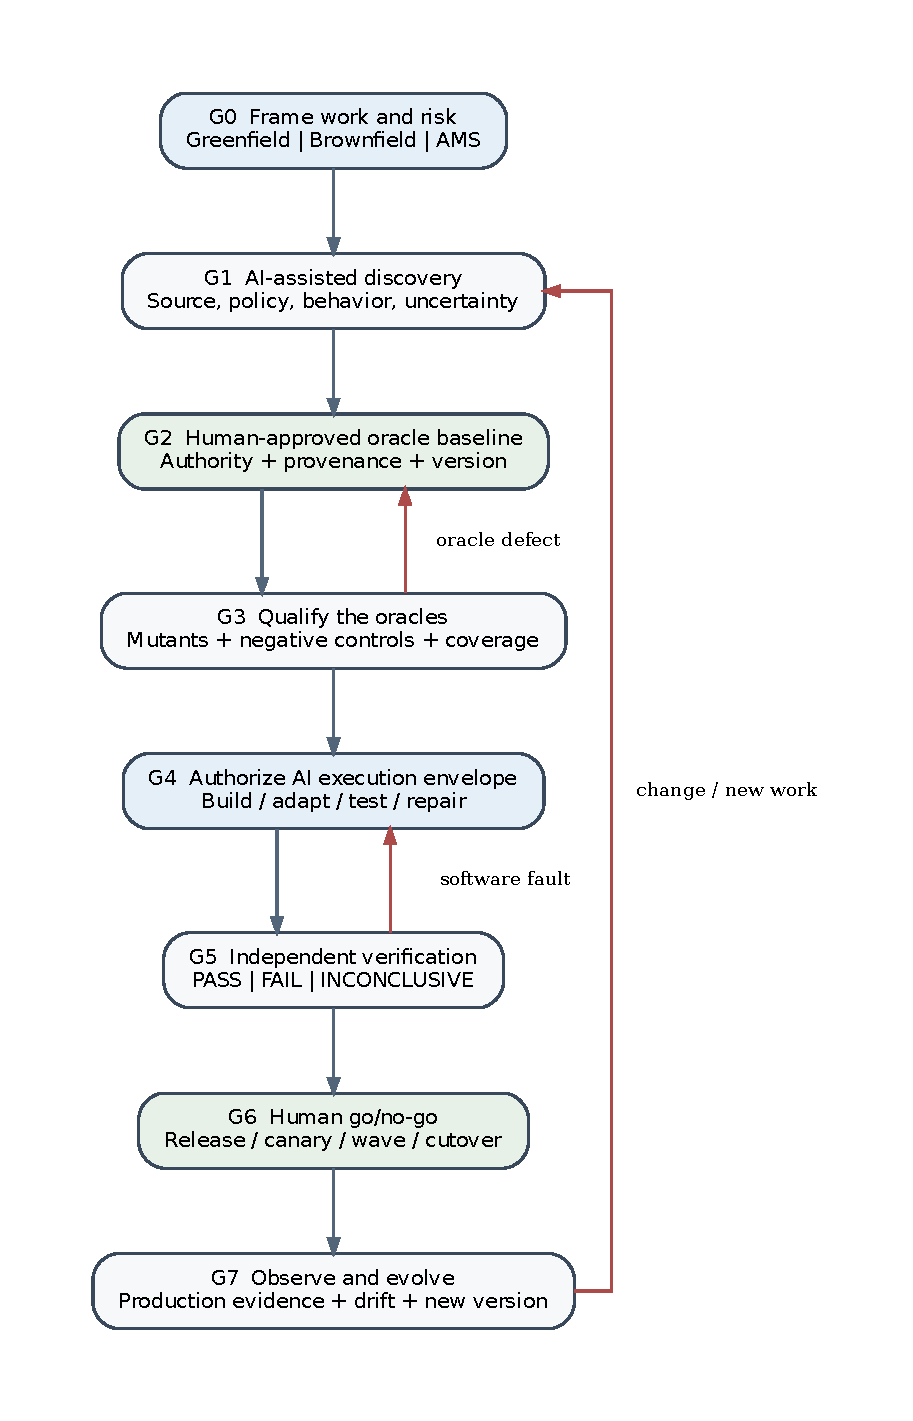
\includegraphics[width=.87\linewidth]{figures/todm_method.pdf}
\caption{The eight TODM gates and principal rework loops. Reverse transitions are deliberate, not methodological failures.}
\label{fig:method}
\end{figure}

\subsection{Stage 0: Frame the unit of work and its risks (G0)}
\textbf{Inputs:} a change request, service incident, legacy modernization target, or new capability. \textbf{Activities:} identify the business capability, owner, scope boundaries, constraints, risk classifications, data sensitivity, operational dependencies, expected quality attributes, and delivery strategy. Separate core behavior from incidental technology. \textbf{Outputs:} \texttt{scope.md}, \texttt{risk-register.json}, a scenario inventory, a system context map, and an evidence-access plan. \textbf{Gate G0:} a named human accountable for business correctness, reviewable scope, observable behavior, and explicit critical risks exist. If not, clarify the scope; do not authorize construction.

\subsection{Stage 1: Discover and discriminate evidence (G1)}
\textbf{Inputs:} signed policies, specifications, APIs, source code, database models, incident logs, runtime traces, and stakeholder interviews as available. \textbf{Activities:} use AI and conventional tooling to extract terms, rules, transitions, decisions, invariants, and unknowns; attach confidence and evidence links. Require human review of inferred, conflicting, legally sensitive, and high-severity rules. \textbf{Outputs:} \texttt{rule-catalog.json}, evidence manifests, a domain glossary, model candidates, a contradiction register, and a coverage map. \textbf{Gate G1:} critical unknowns are either resolved or explicitly classified as unresolved with accountable owners and stop conditions. The system must not equate high model confidence with authoritative acceptance.

\subsection{Stage 2: Specify, review, and freeze a baseline (G2)}
\textbf{Activities:} translate reviewed requirements into typed machine-readable contracts, preferably standards-based where the chosen adapter can enforce a declared semantic subset. Attach rule ownership, effective dates, versions, example boundaries, permissions, and required runtime observation fields. Hold a human approval review that can reject or revise generated oracles. \textbf{Outputs:} baseline manifest, approved model files, an audit record, and version/hash references. \textbf{Gate G2:} no critical oracle is unowned, no unresolved contradiction is concealed, and authorized approval matches the exact signed version. If a contract needs modification later, issue a new reviewed baseline rather than editing the old one in place.

\subsection{Stage 3: Qualify the judges (G3)}
\textbf{Activities:} challenge oracles with known-correct cases, boundary values, deliberately faulty candidates, mutation operators, stale-data scenarios, missing observations, and runtime evaluator failures. Measure false alarms and missed faults; test evidence ordering, idempotence, authorization leakage, and baseline tampering. Distinguish \emph{test quality} from \emph{oracle semantic correctness}. \textbf{Outputs:} qualification suite, mutant catalog, witnessed results, and coverage/uncertainty report. \textbf{Gate G3:} all designated critical seeded violations are detected in the qualification suite, known-correct controls pass, and missing evidence causes \INC{}, never an accidental pass. A failure returns to Stage 2 or 3, depending on whether the contract or implementation of the oracle is at fault.

\subsection{Stage 4: Delegate bounded implementation (G4)}
\textbf{Activities:} create a construction mandate and allow tools/agents to design, implement, generate tests, refactor, migrate data, and repair within its bounds. Adopt SDD, TDD, BDD, formal development, or standard engineering practices as useful. Agents may request baseline amendments but cannot approve them. \textbf{Outputs:} reproducible candidate build, source commit, dependency manifest, generated test reports, runtime observability bindings, and agent execution logs. \textbf{Gate G4:} the candidate is reproducible, the mandate is respected, and construction evidence is complete enough for independent observation. Otherwise, repair within the mandate or escalate an out-of-scope requirement.

\subsection{Stage 5: Run independent verification (G5)}
\textbf{Activities:} bind candidate outputs, APIs, process events, case states, decision inputs, data records, and relevant static-analysis observations to the approved baseline. The verification plane must execute independently from agent-generated TDD/BDD tests. Use differential, metamorphic, property-based, process-conformance, security, and other assessments when pertinent. \textbf{Outputs:} per-oracle verdicts, reproduced execution traces, counterexamples, and an aggregate release decision. \textbf{Gate G5:} no critical \FAIL{} or \INC{} remains for the selected release scope; required oracles were actually executed; evidence is complete and attributed to the intended candidate and baseline. A software violation returns to Stage 4. An oracle defect or genuine business ambiguity returns to Stage 2/3 for human adjudication.

\subsection{Stage 6: Authorize controlled delivery (G6)}
\textbf{Activities:} a human accountable party examines residual risk, oracle execution coverage, critical exclusions, incident response, rollback/compensation feasibility, and deployment change windows. Choose release unit: feature flag, canary, per-capability wave, parallel run, or single cutover. \textbf{Outputs:} a human go/no-go decision, release manifest, migration/reconciliation checks, and operational handover. \textbf{Gate G6:} authorized go decision refers to exact baseline and candidate versions, evidence, and deployment mode. Even a clean oracle report is not a substitute for authorization in high-impact releases.

\subsection{Stage 7: Observe, learn, and version (G7)}
\textbf{Activities:} monitor production behavior, false positives, unanticipated states, incident rates, policy changes, drift, and evidence freshness. Introduce new rule candidates from observed anomalies without treating observations as automatically correct. \textbf{Outputs:} conformance trends, change proposals, incidents, baseline evolution history, and a new work backlog. \textbf{Gate G7:} the operational service has assigned ownership and alert action paths. A change in business policy restarts baseline review; a software defect can trigger a bounded repair; a new business capability restarts Stage 0.

\begin{table}[htbp]
\centering\small
\caption{Forward, repair, and escalation semantics at each gate. ``Hold'' prevents a false success when evidence is missing.}
\begin{tabularx}{\linewidth}{@{}lX X@{}}
\toprule
Gate & Sufficient evidence to advance & On failure / missing evidence \\
\midrule
G0 & accountable scope, owner, risks & clarify scope; hold \\
G1 & traced rules and surfaced unknowns & investigate evidence; hold \\
G2 & signed exact baseline version & human review; return to discovery \\
G3 & seeded faults killed, controls pass & fix oracles; repeat qualification \\
G4 & reproducible candidate and mandate compliance & autonomous repair or escalate \\
G5 & applicable critical controls pass with evidence & repair candidate or reopen baseline \\
G6 & explicit human release authorization & no-go, limit blast radius, or delay \\
G7 & alerts, ownership, and evolution record & incident process / new controlled change \\
\bottomrule
\end{tabularx}
\label{tab:gates}
\end{table}


\section{Operational Controls and Responsibility Assignment}
\subsection{Roles and separation of duties}
TODM distinguishes \emph{who may propose}, \emph{who may approve}, \emph{who may implement}, and \emph{who may certify the evidence}. One human can hold several roles in a small project only when independence requirements remain meaningful and documented; for critical changes, the person approving the business interpretation should not be acting merely as a proxy for the implementing agent. No committee size is prescribed.

\begin{table}[htbp]
\centering\footnotesize
\caption{Illustrative authorization matrix. P: propose; A: approve; E: execute; R: review. Dashes mean no unilateral authority.}
\begin{tabularx}{\linewidth}{@{}p{28mm}cccccX@{}}
\toprule
Role & Discover & Baseline & Oracle QA & Build & Release & Accountability \\
\midrule
Domain owner & R & A & R & -- & A & business meaning and acceptable risk \\
AI analyst & P & P & P & -- & -- & evidence proposals; no sign-off \\
Oracle steward & R & P & E & -- & R & model validity and independent qualification \\
AI builder & -- & -- & -- & E & -- & candidate implementation under mandate \\
Verifier service & -- & -- & E & -- & -- & reproducible findings, no normative edits \\
Release owner & -- & -- & R & R & A & rollout and operational continuity \\
\bottomrule
\end{tabularx}
\label{tab:roles}
\end{table}

\subsection{A non-bypassable policy for verdicts}
Release gating must be encoded as a deterministic control, not summarized by an LLM in free text. A pipeline can collect many kinds of evidence, but its final decision follows a small set of rules. The following pseudocode captures the intended ordering and shows that human authorization is distinct from oracle success.

\begin{lstlisting}[caption={Normative gate policy, expressed as pseudocode.},label={lst:gate}]
function evaluateRelease(candidate, baseline, scope):
    if not verifyApprovedBaseline(baseline):
        return HOLD("unverified baseline")
    required = applicableCriticalOracles(baseline, scope)
    if required is empty and scope.hasCriticalRisks:
        return HOLD("critical risks lack controls")
    outcomes = runIndependentEvaluators(required, candidate)
    if any(outcome == FAIL for outcome in outcomes):
        return BLOCK_WITH_COUNTEREXAMPLES
    if any(outcome == INCONCLUSIVE for outcome in outcomes):
        return HOLD_FOR_EVIDENCE
    if not traceabilityComplete(outcomes, candidate, baseline):
        return HOLD_FOR_EVIDENCE
    return ELIGIBLE_FOR_HUMAN_GO_NO_GO
\end{lstlisting}

The pseudocode models a \emph{conservative} default gate. For noncritical findings the release owner can record a scoped, dated acceptance of residual risk; such exceptions are visible and cannot mutate an underlying critical oracle. An emergency release follows a separately approved emergency path with compensating controls rather than spoofing a successful evaluation.

\subsection{Evidence record and immutable linkage}
A verification record minimally identifies: candidate commit and build digest; oracle baseline version and integrity digest; model profile and evaluator version; exact input or event correlation identifier; timestamp and environment; raw observation pointer; verdict; counterexample if any; and the approving owner for any exception. Since an event stream can be partially delivered, the evaluator must explicitly define a completeness or watermark criterion before reporting \PASS{} for order-dependent properties. Cross-system clocks and correlation identifiers require particular care during incremental modernizations.

\subsection{Failure taxonomy and routing}
TODM separates \emph{implementation deviation}, \emph{oracle implementation defect}, \emph{business-semantic disagreement}, \emph{unsupported model construct}, \emph{missing evidence}, \emph{evaluator outage}, and \emph{baseline-integrity violation}. Each requires a different action. Only implementation deviation is automatically routed to the construction agents. Oracle defects return to oracle qualification; semantic disagreement requires the accountable domain owner; unsupported constructs and missing evidence hold the release until the declared requirements are met. Baseline integrity violation blocks evaluation until independent revalidation. This routing prevents ``repairing'' a missing capability by weakening the rule intended to detect it.

\section{Agent Governance Alignment: Authority Is Not Correctness}
\subsection{Two distinct assurance questions}
A coding agent may have a valid mandate to change a service yet produce an implementation that violates an approved business rule. Conversely, an implementation may satisfy every applicable behavioral oracle while having been produced through an unauthorized action, for example by reading restricted data or bypassing a required review. These failures are independent. TODM therefore distinguishes two predicates:
\begin{equation}
  \operatorname{Authorized}(a,M,E) \quad\text{and}\quad
  \operatorname{Conformant}(x,B_v,\mathcal{O}),
\end{equation}
where $a$ is an action, $M$ is its human-approved mandate, $E$ is the execution context, $x$ is the candidate's observable behavior, $B_v$ is the approved oracle baseline, and $\mathcal{O}$ is the applicable evidence set. Authorization concerns \emph{who may do what, where, and for how long}; conformance concerns \emph{whether the resulting behavior satisfies the approved contracts}. A release is eligible for human consideration only when both checks succeed and the evidence is sufficient.

\begin{table}[htbp]
\centering\small
\caption{Authority and behavioral correctness are independent dimensions. A passing oracle cannot retroactively authorize an action.}
\begin{tabularx}{\linewidth}{@{}p{28mm}p{30mm}X@{}}
\toprule
Action authorization & Oracle verdict & Mandatory disposition \\
\midrule
Authorized & \PASS{} & Eligible for the separate release authorization gate; not automatically deployed. \\
Authorized & \FAIL{} & Block candidate; repair under the mandate or escalate a contract dispute. \\
Unauthorized & \PASS{} & Block and investigate the authority breach even if the resulting software behaves correctly. \\
Unauthorized & \FAIL{} or \INC{} & Block; investigate both the mandate violation and the missing or negative behavioral evidence. \\
\bottomrule
\end{tabularx}
\label{tab:authority}
\end{table}

\subsection{Constitutional and polycentric governance as a complementary layer}
The author's related \emph{constitutional and polycentric agent governance} (CPAG) framing, discussed in the non-peer-reviewed companion essay \emph{De Leviat\'an al Autopilot}\footnote{Author's companion essay (2026): \url{https://jmfloreszazo.com/de-leviatan-al-autopilot/}. This conceptual essay is not independent empirical validation of CPAG or TODM.}, asks how agents receive mandates, how responsibilities are separated, and how authority is monitored and revoked. TODM answers a narrower question: how to establish and execute independently approved behavioral acceptance conditions for software that agents produce or change. The two proposals are conceptually compatible but not interchangeable. CPAG is \emph{not} a mandatory runtime, certification, standard, or prerequisite of TODM; nor is this paper an empirical validation of CPAG. An external authorization system can provide mandate decisions and revocation events to TODM through a stable interface. An organization can implement the same authority separation through ordinary repository permissions, protected branches, CI policies, and accountable human review.

The following cross-system invariants make the boundary testable: (I1) no construction identity can approve a baseline it proposes; (I2) each verification record identifies the mandate and the baseline used; (I3) revocation prevents new delegated execution and blocks promotion until a fresh authorization is established; (I4) a \PASS{} verdict cannot override an authorization denial; and (I5) a mandate grant cannot override a critical \FAIL{} or \INC{} verdict. These are design requirements that need implementation and testing, not established results.

\subsection{A worked two-plane governance failure}
Consider the approved EUR~10,000 authorization rule. The implementation agent is explicitly permitted to change the approval service but not the approved rule. If it introduces a EUR~12,000 threshold, its code change can be \emph{authorized} while its output is \emph{nonconformant}: a EUR~11,000 request is incorrectly auto-approved. The independent DMN or typed decision oracle blocks promotion. Conversely, an agent that reads unauthorized customer records to produce a perfectly conformant implementation has committed a mandate violation; TODM's successful business verdict cannot erase that breach. This distinction prevents a common category error: treating code correctness as sufficient proof of legitimate agent behavior.

\subsection{Interfaces, responsibilities, and non-goals}
A minimal governance integration passes a \texttt{mandateId}, \texttt{principalId}, \texttt{scope}, \texttt{expiresAt}, \texttt{baselineDigest}, and \texttt{authorizationDecision} to the release policy, and records them alongside independent oracle verdicts. The authorization service owns identity, privilege, policy exceptions, and revocation. The TODM verification service owns the observable bindings, declared oracle semantics, verdicts, and counterexamples. Human owners retain authority to approve the normative baseline and production decision. Neither service may silently mutate the other's authoritative record. The architecture can integrate with an ontology or dependency graph for impact analysis, but such a graph is advisory context rather than a substitute for either authorization or correctness evidence.

\section{Adoption Criteria and Methodological Conformance}
An organization may implement TODM with a few scripts or a larger platform. A system is \emph{TODM-conformant at the process level} only if the following demonstrable conditions hold: a named human authority establishes normative rules; each release names an immutable baseline; construction agents cannot unilaterally approve baseline changes; the selected applicable oracles have executable evaluators and qualification evidence; evidence-incomplete conditions are distinct from pass; failures route to explicit recovery paths; and the final production decision is owned by an authorized human. This process-level statement is \emph{not} a certification program or claim of compliance with any OMG standard.

The method may be tailored in proportionality but not in its safety invariants. When a particular domain has no meaningful automated oracle, the process explicitly admits the gap and uses human evaluation with recorded criteria rather than pretending the gap was tested. A project that generates diagrams but never runs them may use TODM vocabulary but should not assert independent oracle-based verification. A project that uses mutation testing only against agent-generated unit tests has a useful test-quality practice, but has not necessarily established independent business authority.

\subsection{Onboarding a small pilot}
A minimum viable pilot can cover a single, observable decision with one responsible business reviewer, a policy excerpt, a versioned JSON/DMN rule, a normal-case and boundary-case suite, a seeded wrong-threshold mutant, and a build agent that cannot edit the approved oracle. Only after this minimal pathway is reproducibly working should teams add cross-cutting process traces, case management, object invariants, and ontology relationships. Expansion is driven by uncovered risk classes and verification evidence, not by a target count of tools or agents.

\section{Reference Architecture: Three Planes and Five Model Families}
The reference architecture in Figure~\ref{fig:planes} separates authority, construction, and verification. A practical implementation needs only file storage, version control, CI jobs, a candidate application, and at least one functioning oracle adapter. Distributed orchestration infrastructure is optional.

\begin{figure}[htbp]
\centering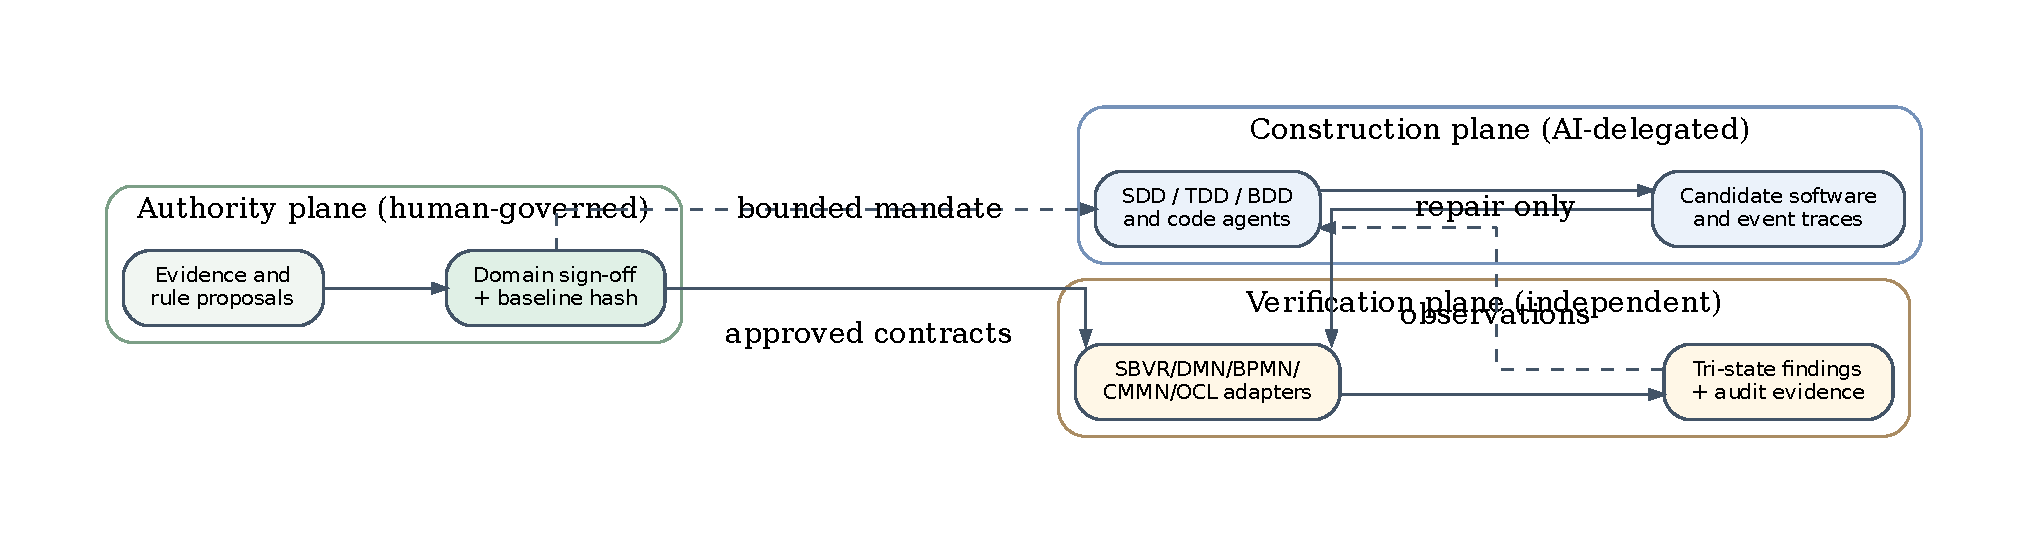
\includegraphics[width=\linewidth]{figures/todm_planes.pdf}
\caption{A tool-neutral three-plane architecture. Protected approval and oracle evaluation are separate from AI construction.}
\label{fig:planes}
\end{figure}

\begin{table}[htbp]
\centering\small
\caption{Risk-selected model families and their executable obligations.}
\begin{tabularx}{\linewidth}{@{}p{13mm}p{29mm}X@{}}
\toprule
Model & Governs & Binding and evidence obligation \\
\midrule
SBVR & Vocabulary and normative business rules & typed terms, business approval, unambiguous operational translation, policy provenance \\
DMN & Input-to-decision logic & typed decision inputs, rule hit policy, expected output, decision trace \\
BPMN & Ordered business activity & correlated events, mandatory activities, allowed paths, sequencing checks \\
CMMN & Case milestones and exceptions & case identity, state transitions, sentries, completion evidence \\
OCL & Invariants and pre-/postconditions & object snapshots, required predicates, scope and evaluator semantics \\
\bottomrule
\end{tabularx}
\label{tab:models}
\end{table}

\textbf{Executability is conditional.} SBVR semantics may be modeled independently from a code generator; its operational mapping must be explicit, typed, reviewed, and tested. OCL expressions require a compatible model and evaluator. BPMN and CMMN XML are not sufficient without correlating the observed process/case events to model elements. DMN decision tables require defined input mappings, hit policies, and expression semantics. Supported model versions and subsets belong in each adapter's conformance manifest. These caveats prevent the category error of claiming that five document types automatically constitute five functioning oracles.

\subsection{An adapter contract}
Let $A_j$ be an adapter for a declared model profile. It must expose (i) model syntax validation, (ii) normalization of event or state input, (iii) deterministic evaluation under pinned versions and configuration, (iv) counterexample/evidence creation, (v) capability limits, and (vi) failure reporting. Adapters may call existing engines or implement constrained profiles; any custom profile must be identified as such and must not be described as full OMG standard conformance.

\subsection{Provenance and optional ontology integration}
A traceability graph links requirement $r$, model node $m$, oracle $o$, runtime observation $x$, source artifact $s$, and verdict $v$. The graph can use existing provenance concepts such as W3C PROV-O \cite{w3c2013prov} and legacy representation standards such as KDM \cite{omg2020kdm}. A sixth, optional ontology module (e.g., an organization-specific knowledge graph) can add dependency mapping, retrieval, and impact analysis. It does \emph{not} independently certify expected behavior, alter verdicts, or own approval authority. No knowledge-graph product or proprietary methodology is required to apply \todm{}.

\section{Machine-Readable Oracle Contracts and Decision Semantics}
\subsection{Minimal artifact schema}
The following JSON is an \emph{illustrative TODM-specific contract}, not an OMG DMN/SBVR encoding. It is intended to clarify the integration boundary; a standards-compliant adapter would additionally retain the underlying normative model file.
\begin{lstlisting}[language={},caption={Illustrative vendor-neutral oracle manifest; not a standardized OMG schema.},label={lst:oracle}]
{
  "id": "AUTH-001",
  "baseline": "approval-1.0.0",
  "evidenceClass": "NORMATIVE",
  "authorityRef": "POLICY-SALES-2026-07",
  "approvalRef": "SIGNOFF-2026-10-20-01",
  "severity": "CRITICAL",
  "profile": "TODM-Decision-1",
  "rule": {
    "field": "request.amountEUR",
    "operator": ">",
    "value": 10000,
    "expected": "HUMAN_REVIEW"
  },
  "requires": ["request.id", "request.amountEUR",
               "decision", "decision.timestamp"],
  "evaluator": "decision-adapter@1.0.0"
}
\end{lstlisting}
This example defines only one side of the decision boundary. A real approved decision model also covers amounts at or below the threshold, null amounts, currency conversion, re-submissions, conflict priorities, and relevant effective dates. Missing those cases should be recorded as explicit incompleteness rather than implicitly approved.

\subsection{Tri-valued semantics}
For candidate $S$, observation set $X$, approved baseline $B_v$, and adapter set $A$, define the per-oracle result
\begin{equation}
R(o,S,X)=\begin{cases}
\FAIL{}, & \text{a supported, applicable rule is violated};\\
\PASS{}, & \text{the rule is exercised and satisfied with valid evidence};\\
\INC{}, & \text{otherwise (missing, ambiguous, or invalid evidence).}
\end{cases}
\label{eq:tristate}
\end{equation}
The three values are not interchangeable. A non-executed control, absent event, timed-out engine, unverifiable model profile, or mismatched baseline hash yields \INC{}, not \PASS{}.

Let $C\subseteq B_v$ be the applicable critical oracles for a scoped release $D$. A conservative gating policy is
\begin{equation}
\operatorname{eligible}(D)=\bigwedge_{o\in C}
\big(R(o,S,X)=\PASS{}\big)\ \land\ \operatorname{integrity}(B_v)\ \land\ \operatorname{evidenceComplete}(D).
\end{equation}
Eligibility is \emph{necessary but not sufficient} for delivery. An explicit human \textsf{GO} decision and any external compliance obligations remain separate. For noncritical oracles, the method permits a documented risk acceptance process, not silent green status.

\subsection{Baseline evolution and anti-tampering}
A baseline change proposes $B_{v+1}$ with a diff, rationale, provenance, affected controls, owner signatures, and requalification evidence. Construction agents receive read-only access to the approved baseline. An ordinary pull request into the constructor's repository must never automatically approve changes to oracle definitions. Independent credentials and protected approval history are recommended. Hashes attest file identity and change detection; they do not validate business truth, nor prevent an authorized human from approving a mistaken rule.

\section{Worked Example: A Shared Specification Error}
Suppose the authoritative business policy states: requests over EUR~10,000 require human authorization before approval or persistence as approved. A generated SDD specification incorrectly sets the review threshold at EUR~12,000; the generated tests confirm EUR~11,000 should be automatically approved.

\begin{table}[htbp]
\centering\small
\caption{Illustrative example; these are reasoned expected outcomes, not experimental results.}
\begin{tabularx}{\linewidth}{@{}p{32mm}X X@{}}
\toprule
Control & Relevant observation & Oracle response \\
\midrule
Specification-based tests & 11,000 automatically approved against 12,000 rule & \PASS{} relative to wrong generated specification \\
SBVR-derived norm & policy defines review above 10,000 & semantic mismatch / re-review \\
DMN decision & 11,000 should yield \textsf{HUMAN\_REVIEW} & \FAIL{} if automatically approved \\
BPMN process & mandatory review event is absent & \FAIL{} with correlated trace \\
CMMN case & case closed without required review evidence & \FAIL{} when case semantics apply \\
OCL invariant & approved state with no authorizing approval & \FAIL{} against object snapshot \\
\bottomrule
\end{tabularx}
\label{tab:example}
\end{table}

\paragraph{Why all five are not always needed.} For a simple stateless API, DMN plus an invariant may suffice. For long-running approvals, process sequencing and case closure become relevant. SBVR provides the governed domain language, but is not intrinsically an executable validator; its approved operational mapping supplies testable predicates. A weak extraction that maps the wrong threshold into \emph{every} oracle can still fail coherently. Independent policy evidence and a knowledgeable approver are essential defenses.

\paragraph{Testing the oracle.} Create mutants setting the threshold to EUR~12,000, omitting the review task, reordering approval after persistence, creating duplicate approvals, and closing an incomplete case. Add negative controls at EUR~9,999 and EUR~10,000, plus malformed and missing-evidence inputs. Record detected mutants, survived mutants, false alarms, and inconclusive outcomes. This is a \emph{protocol design}, not a claim that a released engine already implements or passes these scenarios.

\section{Application Profiles}
\subsection{Greenfield development}
For a new application, the authoritative knowledge is primarily the newly approved policy, stakeholder decisions, constraints, and examples. No legacy system exists to serve as a differential reference. Thus the method emphasizes human-reviewed normative baselines, boundary property tests, scenario elicitation, contract completeness, non-functional evidence, and explicit unknowns. After G2, agents can implement autonomously within a mandate. A newly generated implementation cannot certify that its own specification is valid.

\subsection{Brownfield modernization}
For a legacy system, TODM starts with characterization of code, data, transaction history, event traces, external contracts, and operational workarounds. It distinguishes \emph{preserve} (approved existing behavior), \emph{correct} (legacy behavior contradicts policy), and \emph{redesign} (deliberately new behavior), all approved before becoming authoritative. Brownfield scope may be deployed as (i) sequential migration waves, (ii) coexisting systems with routing rules and reconciled states, or (iii) a single cutover. During coexistence, cross-system consistency, at-most-once effects, data authority, and inter-system contract violations require additional oracle checks. A single cutover requires rehearsed reconciliation and post-cutover contingency: ``rollback'' alone cannot account for data written after the switch.

\subsection{Application Management Services (AMS)}
For maintenance, incidents, security fixes, and change requests, use existing baselines as regression contracts. New production observations and support tickets enter Stage 1 as \emph{observed} evidence; only approved changes amend normative behavior. The method supports patch verification, recurring conformance monitoring, operational invariant alerts, controlled hotfixes, and drift detection. A critical incident can shorten the normal review cycle only through a documented emergency governance path, followed by retrospective baseline reconciliation.

\subsection{A shared core, variable iteration size}
Across all profiles, the invariant elements are authority separation, baseline integrity, oracle qualification, tri-valued evaluation, and human decision rights. The difference is the source of truth, selected behavioral dimensions, observability binding, and deployment granularity. \todm{} does not prescribe Scrum, Kanban, waterfall, a specific cloud, or a particular coding model.

\section{Quality Metrics and Falsifiable Research Questions}
This paper deliberately excludes economic claims and cost KPIs. The evaluation concerns behavioral correctness, independent fault detection, evidence integrity, governance, reliability, and engineering autonomy. Numerical thresholds below are \emph{candidate acceptance thresholds for future studies}, not observed performance.

\begin{table}[htbp]
\centering\footnotesize
\caption{Operational metrics. Denominators and exclusions must be declared before evaluation.}
\begin{tabularx}{\linewidth}{@{}p{39mm}X@{}}
\toprule
Metric & Operational definition and interpretation \\
\midrule
Critical rule coverage & Applicable critical rules with executed evaluators divided by all approved applicable critical rules. Disclose exclusions. \\
Oracle mutation detection (OMD) & Correctly detected non-equivalent, executed seeded faults divided by all non-equivalent, executed faults. Disclose unexecuted mutants. \\
False-positive rate (FPR) & Known-correct controls flagged \FAIL{} divided by all known-correct controls executed. \\
Inconclusive rate (IR) & Applicable oracle attempts returning \INC{} divided by all applicable attempts; separate data loss from evaluator failure. \\
Traceability completeness & Issued verdicts linked to rule, evidence, build and baseline divided by all issued verdicts. \\
Escaped defect density & Confirmed production defects per predefined capability or change unit, stratified by severity and exposure. \\
Human approval integrity & Baseline changes with independent recorded approval divided by all changes. \\
Mandate conformance & Delegated actions within approved scope and validity divided by all observed delegated actions; report unknown/unobserved actions separately. \\
Revocation enforcement & Attempts to execute or promote after mandate revocation that are correctly blocked divided by all controlled revocation test attempts. \\
Autonomous accepted work share & Eligible accepted work items completed without direct human code edits divided by all eligible accepted items. \\
Repair convergence & Detected candidate violations subsequently repaired and reverified within the mandate; report unresolved items and iteration count. \\
\bottomrule
\end{tabularx}
\label{tab:metrics}
\end{table}

\textbf{Research questions.} RQ1 asks whether separately approved oracles reveal shared-specification faults missed by tests derived from the same generated specification. RQ2 asks whether mutation-qualified baselines reduce oracle false confidence, compared with unqualified models. RQ3 asks whether the approach generalizes across greenfield, brownfield, and AMS. RQ4 asks whether bounded autonomy maintains acceptance quality without unauthorized baseline edits. RQ5 examines how frequently human review reverses the AI-derived interpretation of business rules. RQ6 asks whether independently enforced mandates prevent unauthorized actions from being accepted even when all behavioral oracles pass.

\textbf{Falsifiable hypotheses.} H1 predicts higher recall for seeded cross-artifact specification errors under TODM than under an otherwise equivalent SDD/TDD/BDD workflow lacking independently approved oracles. H2 predicts lower false-positive and inconclusive rates after oracle qualification when compared under the same evaluation set. H3 predicts fewer unauthorized baseline changes under protected approval control than under agent-writable baselines. H4 predicts that at least some work scopes achieve a higher share of independently accepted autonomous work without increasing critical escaped defects. H5 predicts that enforcing the independent authorization and conformance predicates prevents release of unauthorized-but-conformant candidates in controlled adversarial tests. These must be tested: a null or adverse result would constrain or refute the corresponding claim.

\section{Proposed Empirical Protocol}
\subsection{Design and comparators}
Use a preregistered mixed-method evaluation with representative, isolated capabilities across greenfield, brownfield, and AMS. For each capability construct two matched pipelines: (A) normal agent-assisted SDD/TDD/BDD with standard CI and human review; (B) the same tools/models/configuration augmented with TODM's independently authorized baseline, oracle qualification, and independent evaluator. Add a third ablation condition without mutation qualification where feasible. For the authority-versus-correctness boundary, include a separate adversarial test condition with deliberately revoked, expired, or over-scoped mandates and otherwise conformant candidates. Rotate conditions across projects and practitioners, control for learning and contamination, and blind independent assessors to pipeline identity.

\subsection{Cases, ground truth, and independence}
Commission domain specialists to label ground truth for business rules from approved documentation, validated scenarios, and adjudicated counterexamples. Seed non-equivalent faults in decisions, event ordering, case closure, state persistence, temporal rules, authorization, and data transformation. Include known-correct decoys to measure false positives. Record each mutant's expected observable effect and verify that the mutant was applied; exclude provably equivalent mutants using a documented adjudication procedure. Preserve a held-out fault set unavailable to generation agents or oracle authors.

\subsection{Sampling, measurement, and analysis}
Determine sample size via a pilot-based power analysis rather than picking a convenient number of runs. Treat repeated runs against the same requirement or repository as correlated observations, not independent projects. Use paired or hierarchical analyses where applicable, publish effect sizes and interval estimates (e.g., bootstrap confidence intervals by project cluster), and report missing evidence separately. Counterbalance model versions and random seeds; version all prompts, code, manifests, tools, data, and evaluator profiles. Security incidents and high-severity faults should be analyzed by severity strata rather than hidden in averaged pass rates.

\subsection{Acceptance before effectiveness}
A prototype first passes engineering acceptance: source compilation, supported-profile parser conformance, baseline tamper tests, missing-evidence behavior, seeded-mutant detection, and human approval audit. Only then can industrial effectiveness be studied. No amount of synthetic demonstration constitutes evidence of reduced production defects or sustained autonomous engineering effectiveness.

\subsection{Reproducibility and reporting}
Publish anonymized cases, model profiles, oracle manifests, non-sensitive traces, mutation operators, study scripts, and a threat-to-validity register subject to intellectual-property and privacy constraints. Report \emph{all} attempted cases, exceptions, exclusions, aborted agent runs, failed baselines, and negative results. Prefer a registered protocol and independent replication to claims based on a single success story.

\section{Executable Research Artifact and Engineering Acceptance}
\subsection{Artifact scope and separation of claims}
A versioned synthetic companion artifact implements an illustrative, deliberately limited subset of the method. It includes five \emph{JSON semantic profiles} associated with SBVR, DMN, BPMN, CMMN, and OCL, a deterministic Python reference evaluator, a C\#/.NET~10 candidate and evaluation scaffold, synthetic greenfield/brownfield/AMS scenarios, fixed mandates, and signed demonstration attestations. The JSON profiles are \emph{not} full implementations of OMG languages, and the artifact is not evidence of standards conformance. Its purpose is to exercise the proposed gate composition and expose falsifiable failure modes, not to validate industrial effectiveness.

\subsection{Reproducible controls and observed synthetic outcomes}
At artifact preparation time, the Python reference runner executed nine baseline/qualification tests, ten signed-assurance tests, and seven additional adversarial release-gate tests. The synthetic fixture suite contains 16 cases: five pass both the behavioral and authority controls and possess the requisite demonstration G6 signature; eleven are blocked. Four deliberately mutated candidates violate at least one oracle family; one deliberately incomplete observation yields \INC{}. These counts describe \emph{selected deterministic engineering acceptance fixtures}, not independently sampled experiments or empirical estimates of defect-detection performance. A fail-closed command-line gate returns success only for a fully passing synthetic signed case, and a nonzero exit status for denied cases. A machine-readable provenance report records the invoked commands, exit codes, and SHA-256 hashes of the baseline and result artifacts.

\subsection{Integrity, authorization, and trust boundaries}
The G2 Ed25519 demonstration signature authenticates the baseline manifest digest, and the manifest binds the model files by hash. The G6 demonstration signature is bound to an individual fixture and that same digest. Consequently, a conformant candidate without a valid G6 attestation remains blocked, as does a signed candidate that fails its oracles or mandate. However, public demonstration keys are not evidence of real human identity; the mandate data is a static unsigned fixture; no production enforcement point, credential revocation service, protected deployment environment, or organizational separation is provided. The evaluator and fixtures also share a repository, so \emph{epistemic independence} is a research objective rather than an established artifact property.

\subsection{Reproduction and research status}
With Python~3.12 or later and OpenSSL with Ed25519 support, the command \texttt{python3 scripts/reproduce.py} runs the deterministic reference and negative controls, failing on unexpected outcomes and writing a JSON reproducibility record. The C\# path is supplied with GitHub Actions configuration for a .NET~10 SDK; compilation and runtime parity are not claimed from the local preparation environment. Independent replication requires a separately trusted business-rule baseline, external assessors, a preregistered comparative design, and a fixed commit or archived release identifier. Until those conditions are satisfied, the paper's effectiveness hypotheses remain \emph{untested}.

\section{Threats, Failure Modes, and Limits}
\paragraph{Oracle circularity.} The same misinterpreted policy can propagate into specifications, code, tests, and all five model files. Logical separation of repositories alone is insufficient; authoritative evidence and human review are necessary, and their own error rates should be studied.
\paragraph{Incomplete models.} A five-model baseline still cannot establish all temporal, security, privacy, performance, and emergent distributed-system properties. Contract coverage must be explicit, and dedicated security or formal verification controls may be required for high-impact systems.
\paragraph{Unsupported language semantics.} BPMN, CMMN, DMN, SBVR, and OCL have nontrivial specifications; translations to JSON, rule snippets, or ad hoc evaluators can lose constructs. Each adapter declares a tested subset. Unknown constructs are \INC{} rather than silently ignored.
\paragraph{Observability gaps.} A model cannot prove a hidden side effect absent sufficient instrumentation. Telemetry may be incomplete or manipulated; evidence provenance and event correlation matter. Static source analysis can identify candidate risks but is not a universal proof of runtime business correctness.
\paragraph{Mandate enforcement can fail.} A correct authorization policy is insufficient if enforcement points are bypassable, revoked credentials remain valid, or telemetry omits delegated actions. TODM does not replace identity governance or security assurance; independent adversarial mandate tests are necessary.
\paragraph{Human authority is fallible.} Approval is an accountability control, not an oracle of absolute truth. Domain experts may disagree or overlook historical exceptions; adjudication, uncertainty recording, and versioned reversals are required.
\paragraph{Changing policy and drift.} Frozen baselines can become obsolete. Effective dates, jurisdictional differences, data migration state, and interactions between coexisting systems must be explicit. Monitoring signals may trigger investigation but not automatic normative reinterpretation.
\paragraph{Scope and generalization.} A single illustrative threshold example is insufficient to establish general effectiveness. AMS emergency changes, asynchronous workflows, probabilistic outputs, and adversarial inputs require dedicated protocols. The 90\% autonomous-work notion discussed in some agentic engineering programs is a possible research target, not an empirically established TODM property.

\section{Research and Implementation Roadmap}
A staged implementation reduces technical risk without requiring five complete standards engines at once. \emph{Milestone M0} constructs the neutral manifest, three-valued verdict format, protected approvals, evidence capture, and reproducible test harness. \emph{M1} implements a DMN or typed decision adapter and a state-invariant evaluator with a narrow OCL-compatible profile. \emph{M2} adds BPMN trace conformance, \emph{M3} adds CMMN case state and milestone controls, and \emph{M4} adds governed SBVR vocabulary with an explicitly reviewed operational mapping. \emph{M5} performs cross-adapter mutation qualification, independent audit, and a multi-profile experiment. A knowledge-graph/ontology adapter may be explored separately after its entity, relationship, and provenance schema have been characterized; it is not a prerequisite for M0--M5.

Every milestone must publish parser/version support, deterministic outputs, qualification tests, sample evidence, known unsupported constructs, and an explicit completion decision. The method should remain implementable by different runtimes and vendors, including plain code repositories and off-the-shelf engines. A branded reference implementation is not evidence that the \emph{methodology itself} is tool-independent; this independence should be confirmed in a cross-platform replication.

\section{Discussion}
TODM reframes AI-assisted software delivery as a problem of \emph{justified acceptance}. Generating an implementation and generating tests both become delegated activities; establishing the conditions under which the resulting software may be called correct remains an accountable, evidence-driven task. Formal and semi-formal models make portions of business intent executable, while human review governs uncertainty and policy changes. The approach is aligned with professional software craftsmanship understood as responsibility for maintainable, well-verified outcomes rather than the volume of code produced.

The method is not a replacement for CI/CD, secure development, SDD, TDD, BDD, domain modeling, incident management, or architectural governance. In particular, a constitutional governance layer determines whether actions are legitimate; TODM determines whether their software outputs satisfy independently authorized behavioral contracts. Both predicates are needed for accountable autonomous delivery. It provides a specific control loop tying these practices to independently governed and qualified oracles. Its additional ceremony should be justified by risk and evidence, not by a demand that every small change instantiate five engines.

\section{Conclusion}
This paper defines \todm{} as a research-ready, tool-agnostic methodology that separates the authority to declare expected behavior from the autonomy to construct software. The methodological core is an approved, qualified oracle baseline; explicit three-plane separation; eight gates with reverse paths; tri-valued verification; and a reproducible evaluation protocol. The proposed design accommodates greenfield, brownfield, and application management without assuming a Big Bang migration, a specific vendor, or the adoption of any particular agent-governance framework. It explicitly separates mandate authorization from behavioral conformance. Its value is plausible but unproven: rigorous comparative studies must establish whether the added independence detects consequential defects and sustains bounded engineering autonomy. Until then, TODM should be read as a falsifiable methodological proposal, not as an experimentally validated quality guarantee.

\section*{Ethics, Transparency, and Author Responsibility}
This manuscript describes a methodology and does not report studies on human participants, production customers, or private repositories. Illustrative values and scenarios are synthetic. Generative AI assistance was used to support drafting, language editing, literature organization, and document production. All technical claims, references, and citations require final human verification prior to submission. The human author is responsible for checking references, the technical claims, the originality and intellectual-property status of the work, and the final submitted version. No AI system is credited as an author.

\section*{Data and Code Availability}
There is no industrial experimental dataset associated with this proposal. The versioned companion artifact (TODM Research Artifact v1.4 (oracle-profile schema v0.4)) provides limited JSON oracle profiles, fixed synthetic cases, a Python evaluator, offline Ed25519 demonstration attestations, a fail-closed command-line gate, and a SHA-256 provenance record. Its engineering acceptance outcomes are not a comparative dataset and do not establish OMG standards conformance, verified local .NET compilation, real human approvals, or industrial effectiveness. The release must be archived with a persistent public identifier and commit hash before external citation as an independently reproducible artifact. The paper's LaTeX source and figures form the reproducible manuscript artifact.

\bibliographystyle{plain}
\bibliography{references}
\end{document}
